\documentclass{article}
\usepackage{amsmath}
\usepackage{amssymb}
\newcommand*{\qed}{\hfill\ensuremath{\blacksquare}}
\usepackage{graphicx}
\graphicspath{{.}}

\title{Computational Linear Algebra, Module 6}
\author{Maya Shende}
\date{Due: March 21st, 2017}

\begin{document}
\maketitle

\begin{enumerate}

\item We can write this linear combination as a set of linear equations, and then solve them for $\alpha$ and $\beta$. 

\item $\overrightarrow{w} - 4\overrightarrow{v} = 
\begin{bmatrix}
	2\\
	-1\\
	1
\end{bmatrix}
- 4
\begin{bmatrix}
	0\\
	1\\
	1
\end{bmatrix}
= 
\begin{bmatrix}
	6\\
	-3\\
	3
\end{bmatrix}
$. So, $\frac{\overrightarrow{w} - 4\overrightarrow{v}}{3} = 
\begin{bmatrix}
	2\\
	-1\\
	1
\end{bmatrix}
$. So, yes, $\overrightarrow{u}$ can be expressed as a linear combination of $\overrightarrow{w}$ and $\overrightarrow{v}$. 

\item We want to find $\alpha$ and $\beta$ such that $
\begin{bmatrix}
	6\\
	1\\
	8
\end{bmatrix}
= \alpha
\begin{bmatrix}
	2\\
	-1\\
	1
\end{bmatrix}
+\beta
\begin{bmatrix}
	0\\
	1\\
	1
\end{bmatrix}
$. By writing out the first equation, we get $6 = 2a \rightarrow \alpha = 3$. So, if we plug this value of $\alpha$ into the second equation, we get $1 = -3 + \beta \rightarrow \beta = 4$. However, when these two values are used in the 3rd equation, we get the $8 = 3 + 4 \neq 7$, which is a contradiction. So, $\overrightarrow{z}$ cannot be expressed as a linear combination of $\overrightarrow{u}$ and $\overrightarrow{v}$. 

\item No, $\overrightarrow{u}$ cannot be expressed as a linear combination of $\overrightarrow{v}$ and $\overrightarrow{z}$:\\ $\alpha
\begin{bmatrix}
	0\\
	1\\
	1
\end{bmatrix}
+\beta
\begin{bmatrix}
	6\\
	1\\
	8
\end{bmatrix}
\neq
\begin{bmatrix}
	2\\
	-1\\
	1
\end{bmatrix}
$\\
Also, $\overrightarrow{v}$ cannot be expressed as a linear combination of $\overrightarrow{u}$ and $\overrightarrow{z}$. 

\item $\alpha_1 r_1 + \alpha_2 r_2 + \dots + \alpha_k r_k = \overrightarrow{0} \rightarrow$ all coefficients must be zero since $r_1, r_2, \dots, r_k$ are all pivot rows and so we know there must be a 1 in a different column of each of these rows. 

\item $\alpha_1 c_1 + \alpha_2 c_2 + \dots + \alpha_k c_k = \overrightarrow{0} \rightarrow$ all coefficients must be zero since $c_1, c_2, \dots, c_k$ are all pivot columns and so we know there must be a 1 in a different row of each of these rows and we also know that all non-one entries must be zero since this is an RREF. 

%exercise 7
\item 
\begin{enumerate}
	\item $v_2$ and $v_4$ are independent, and $v_1$ is a linear combination of $v_2$ and $v_4$, not $v_2$ alone, so $v_1$ and $v_2$ are independent. 
	\item We know that $v_3 = v_2 + v_4$ and $v_2 = v_1 + v_4$ from above. So, rearranging the second equation gives us $v_4 = v_2 - v_1$. Now, if we replace $v_4$ in the equation for $v_3$, we have $v_3 = v_2 + (v_2 - v_1) = -v_1 + 2v_2$. \qed
	\item We have $v_1 = v_2 - v_4$ from above, and if we rearrange this, we have $v_4 = -v_1+ v_2$. 
	\item We know $v_5 = 3v_2 - v_4$ and $v_4 = v_2 - v_1$ from above. Now, if we replace $v_4$ in the first equation by our second equation, we have $v_5 = 3v_2 - (v_2 - v_1) = v_1 + 2v_2$. 
\end{enumerate}

%exercise 8
\item Suppose $v_1, v_2, \dots, v_n$ are independent. Then, by definition we know that\\
$a_1v_1 + a_2v_2 + \dots + a_nv_n = 0$ if $a_1 = a_2 = \dots = a_n = 0$. Now, choose a subset of $k$ vectors and suppose by way of contradiction that these $k$ vectors are not independent. Then we have\\
$a_1v_1 + a_2v_2 + \dots + a_iv_i + \dots + a_kv_k = 0$, but $a_i \neq 0$. Now, let's add back the $n-k$ vectors with coefficients of zero (so these vectors will effectively not contribute to the sum) and we get\\
$a_1v_1 + a_2v_2 + \dots + a_iv_i + \dots + a_kv_k + \dots + a_nv_n = 0$, but $a_i \neq 0$, a contradiction. Therefore, any subset of the original set of independent vectors must also be independent. \qed

%exercise 9
\item The span of these vectors seems to be along a diagonal plane. 

%exercise 10
\item The span of just the two vectors is the same as the span of all 3 vectors. This is because the 3rd vector is linearly independent on the first 2 vectors. The span of just $\overrightarrow{u}$ by itself is just a straight line, and it is not the same as the span of any of the other vectors. 

%exercise 11
\item $\overrightarrow{u}$ and $\overrightarrow{v}$ will span the same set. They span the set of all 2-dimensional vectors in the x-y plane. 

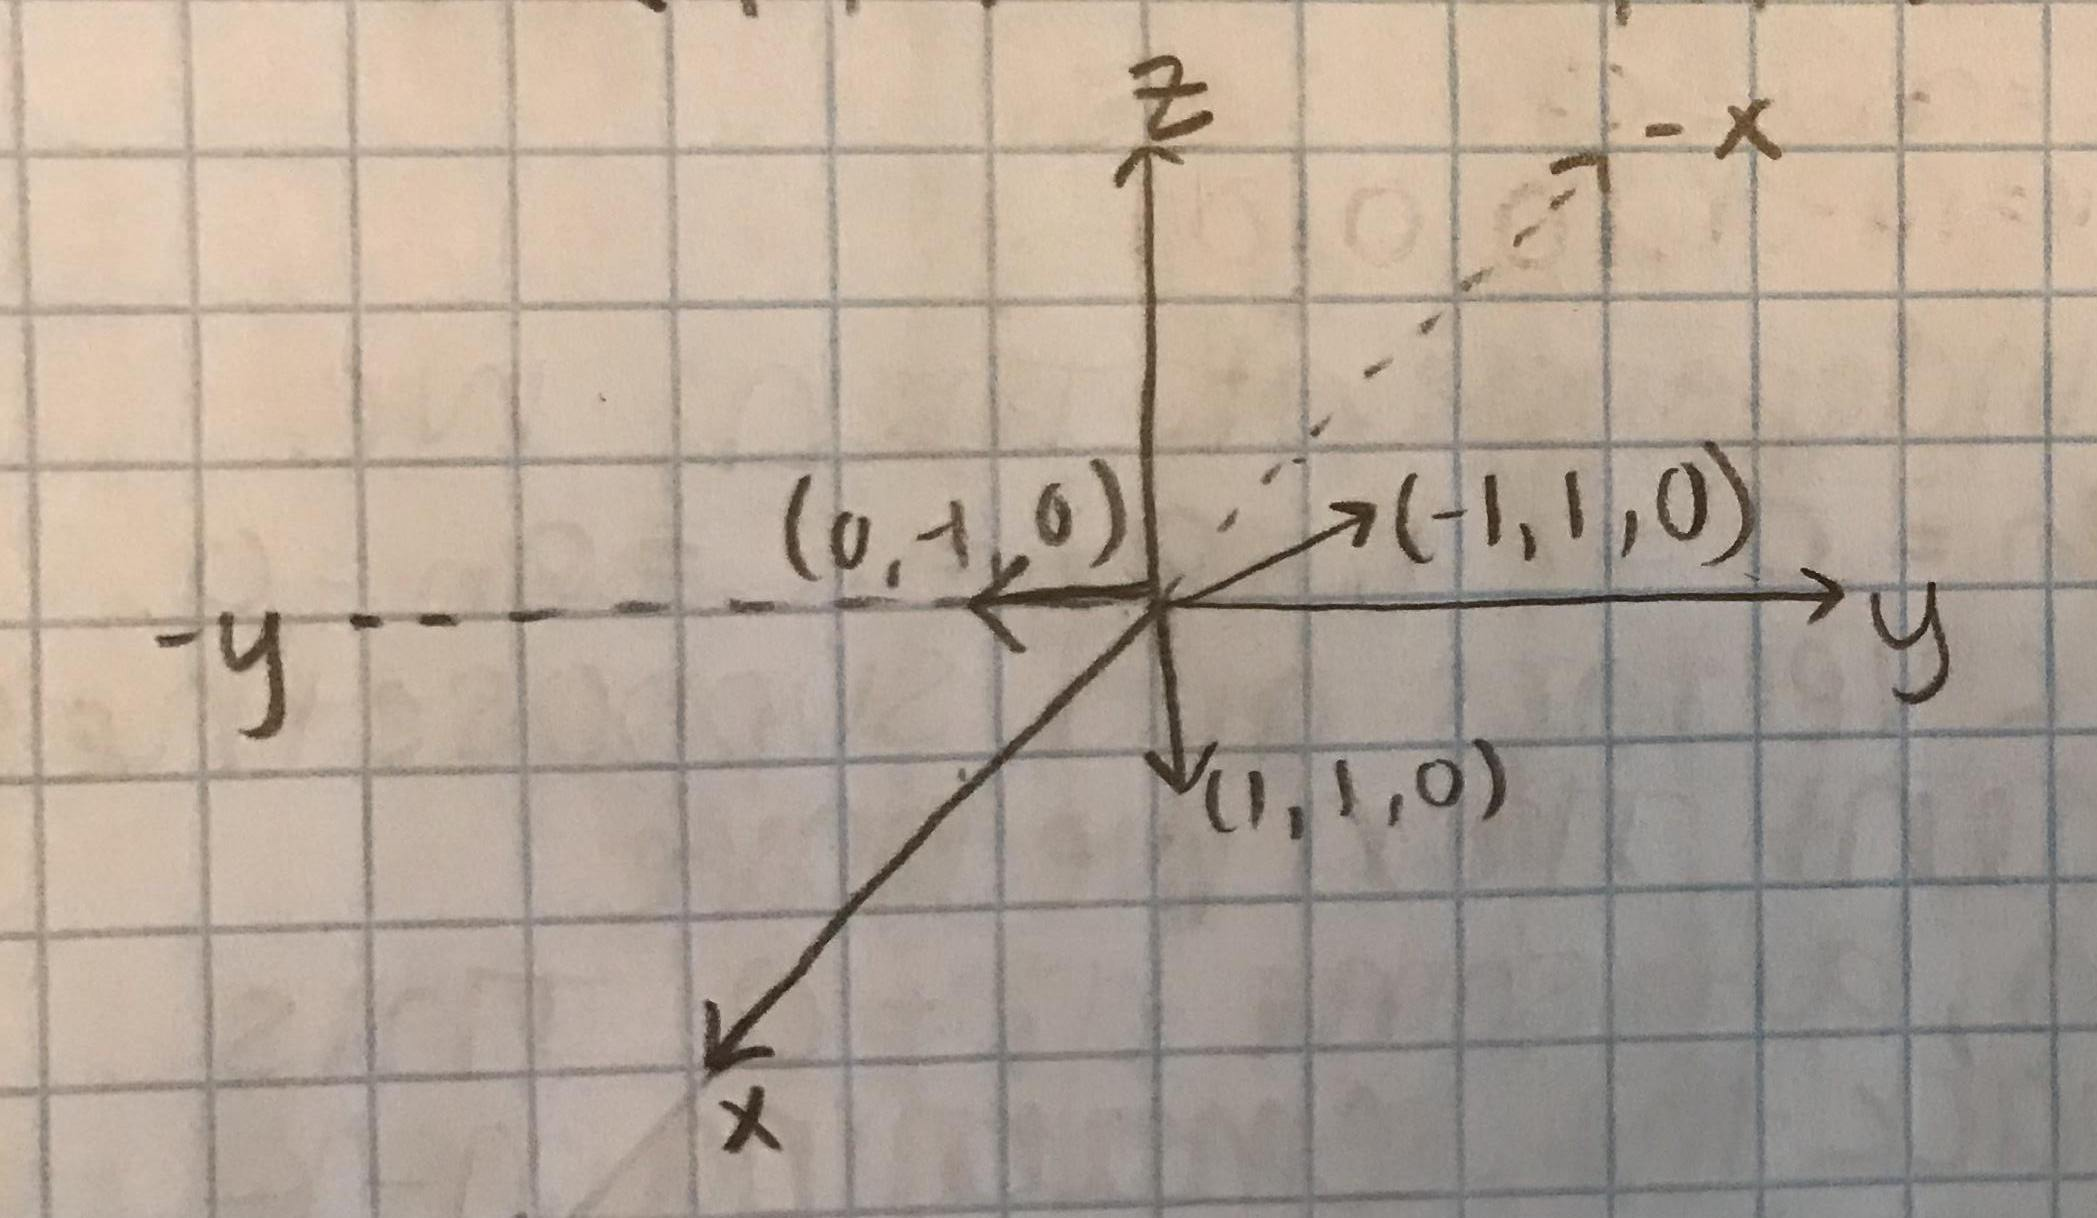
\includegraphics[scale=0.1]{exercise11.jpg}

%exercise 12

\item No single vector can generate the x-y plane because there needs to be at least one vector per component, and there are two components in the x-y plane. So, at least 2 vectors are needed to generate this plane. 

%exercise 13
\item To show that $\overrightarrow{u}$ and $\overrightarrow{v}$ are independent, we must show that\\
$\alpha \overrightarrow{u} + \beta \overrightarrow{v} = \overrightarrow{0}$ only if $\alpha = \beta = 0$. So, $
\alpha 
\begin{bmatrix}
	1\\
	1\\
	0
\end{bmatrix}
+ \beta 
\begin{bmatrix}
	-1\\
	1\\
	0
\end{bmatrix}
= 
\begin{bmatrix}
	0\\
	0\\
	0
\end{bmatrix}
$. So, we have the equations $\alpha - \beta = 0$ and $\alpha + \beta = 0$. Therefore, the only way this can hold true is if both $\alpha$ and $\beta$ are 0. Therefore, $\overrightarrow{u}$ and $\overrightarrow{v}$ are independent. \qed

To show that $\overrightarrow{w}$ is a linear combination of $\overrightarrow{u}$ and $\overrightarrow{v}$, we must find an $\alpha$ and $\beta$ such that:\\
$
\alpha 
\begin{bmatrix}
	1\\
	1\\
	0
\end{bmatrix}
+ \beta 
\begin{bmatrix}
	-1\\
	1\\
	0
\end{bmatrix}
= 
\begin{bmatrix}
	0\\
	-1\\
	0
\end{bmatrix}
$. So, we can see that our equations are $\alpha - \beta = 0$ and $\alpha + \beta = -1$, leading us to find that $\alpha = \beta = -\frac{1}{2}$. 

%exercise 14
\item Suppose $span(v_1, v_2, \dots, v_n)$ has dimension $n$, and for some $i \leq n$, $v_i$ is dependent on the others. This means the remaining $n-1$ vectors can generate the same span as all $n$ vectors, so the dimension is actually $n-1$, a contradiction. Therefore, the $n$ vectors are linearly independent. \qed

%exericise 15
\item 
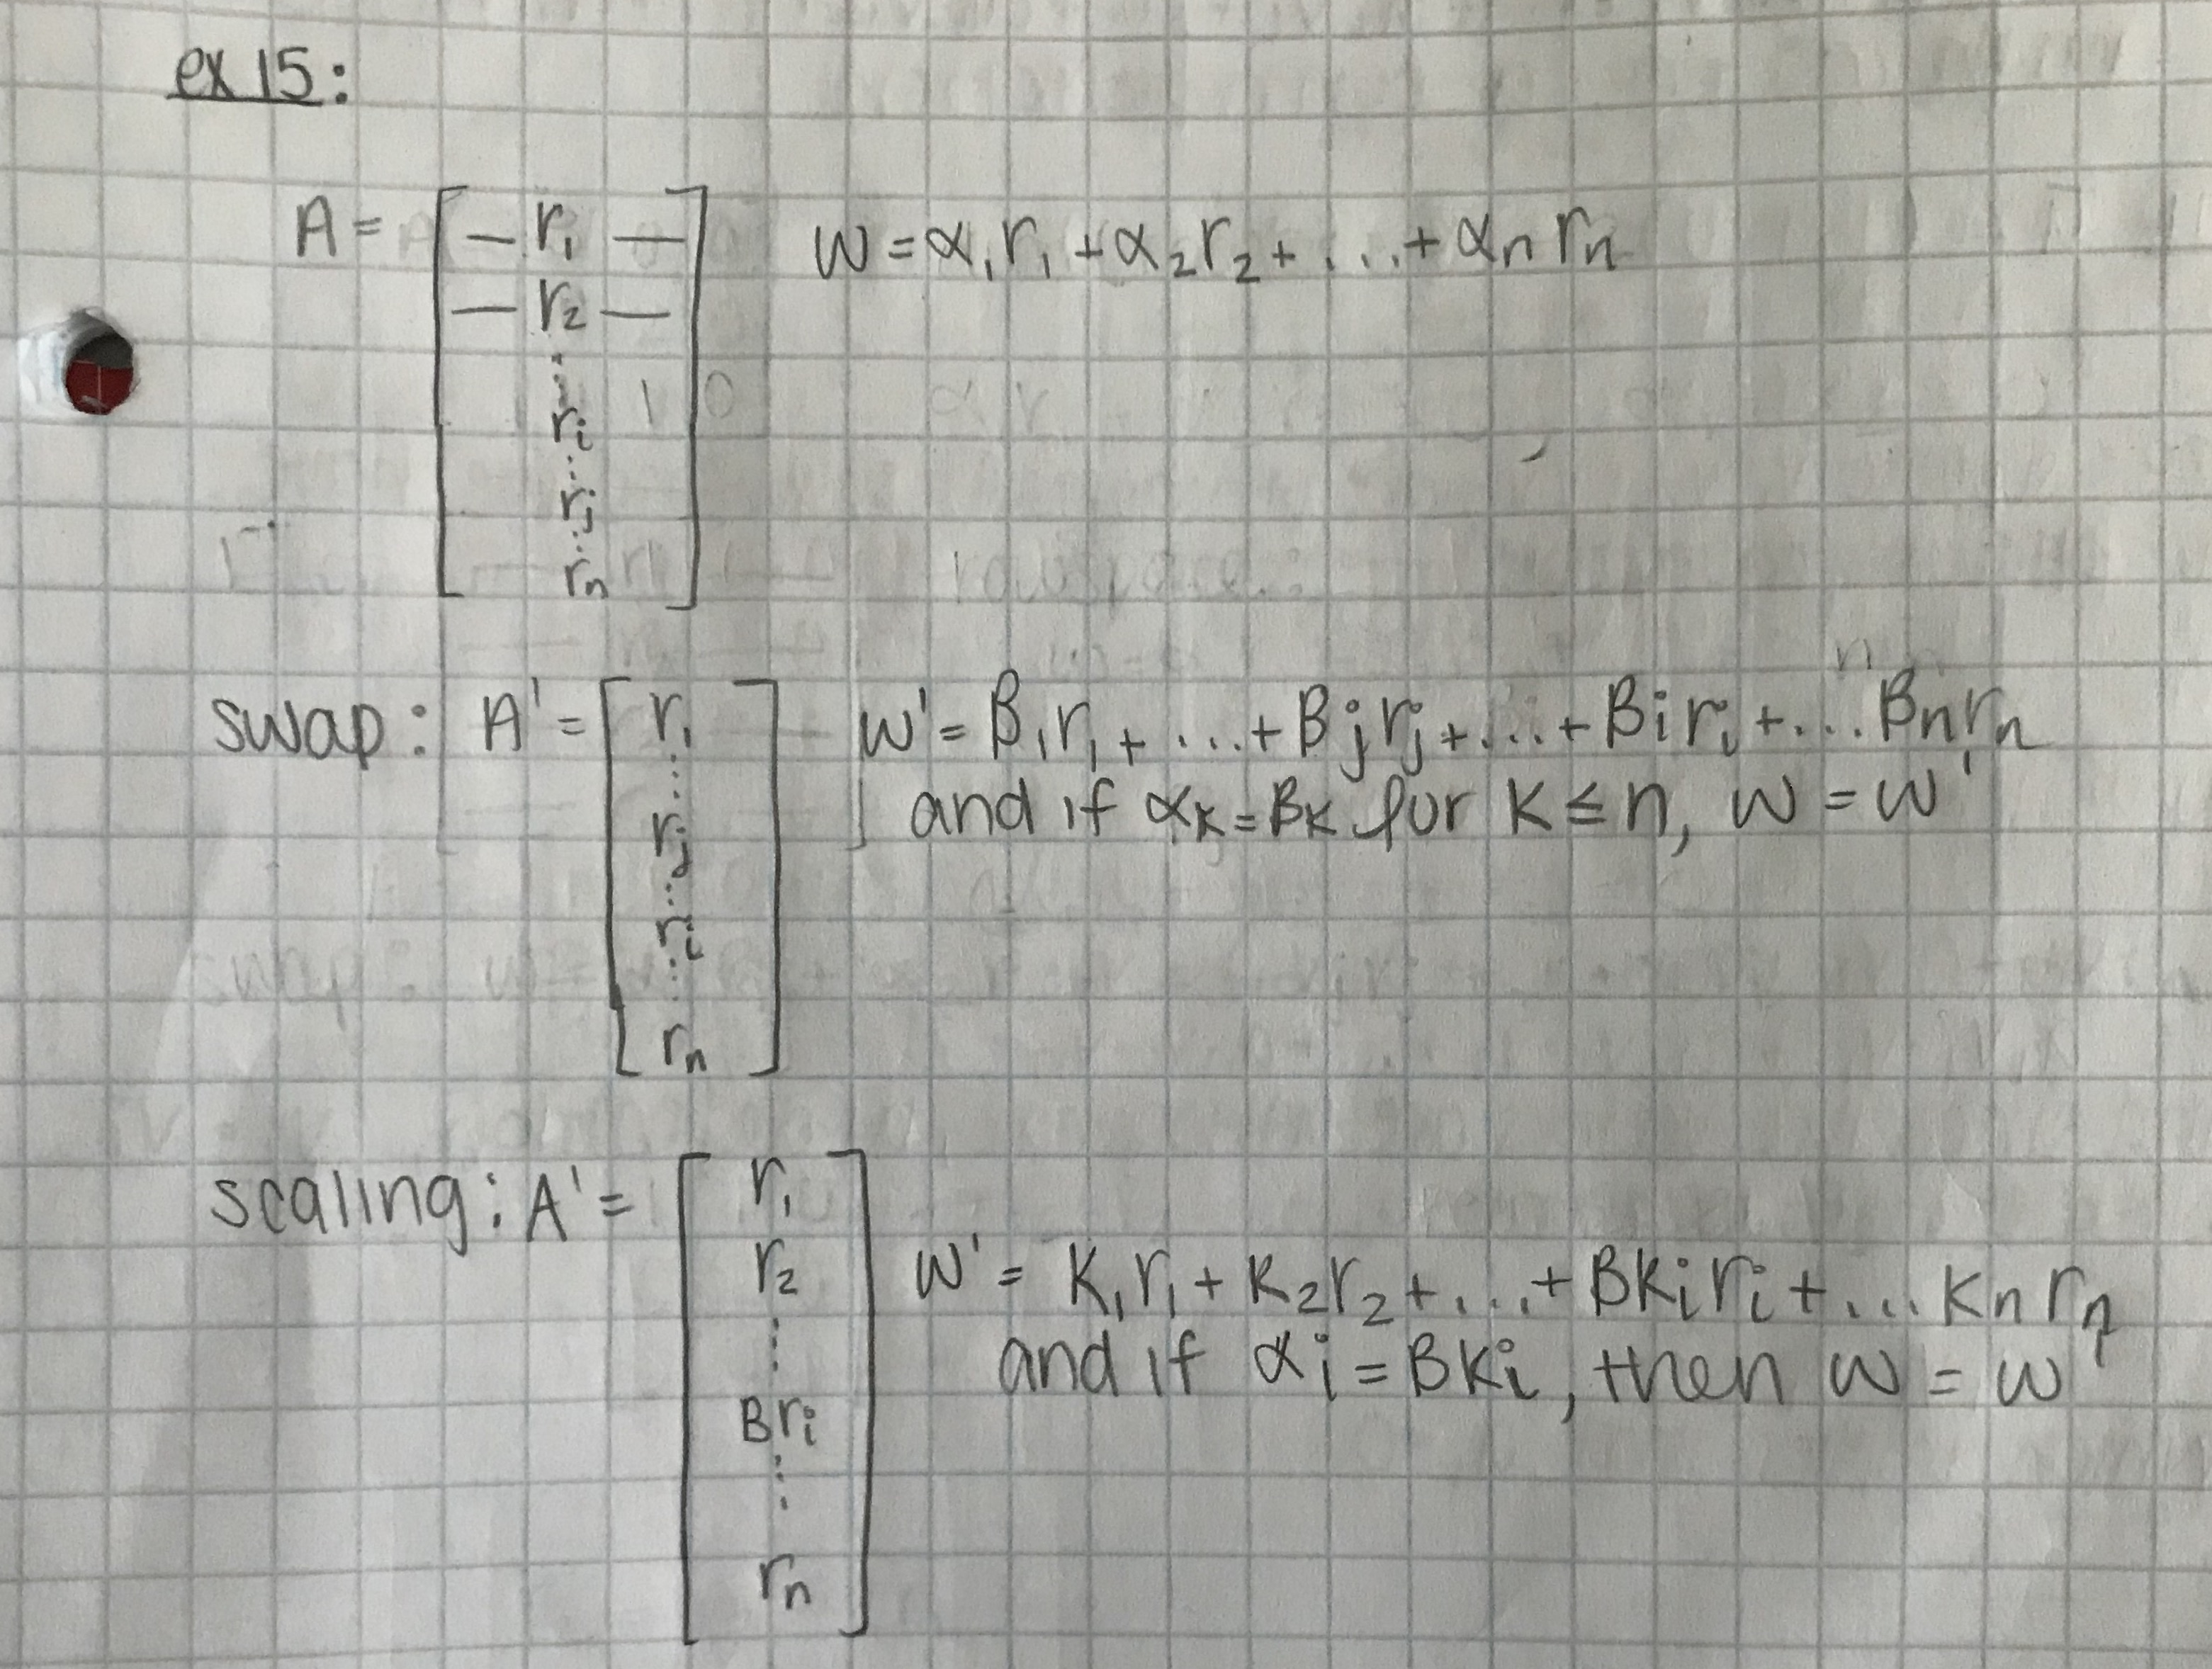
\includegraphics[scale=0.1]{exercise15}

%exercise 16
\item The pivot rows are independent because through the process of developing the RREF, we ensure that each of these rows has a 1 in some column, and no other row has a 1 in that same column, and all non-pivot entries are zero. Therefore, no combination of pivot rows can make another pivot row. 

%exercise 17
\item In class, we showed that $dim(rowspace(A)) = dim(colspace(A))$. We also know that in an RREF, the rank of a matrix is equal to the number of pivots, or the number of pivot rows, also called the dimension of the rowspace of that matrix. So, if we put all of this together, we have \\
rank = number of pivots in RREF = number of pivot rows = $dim(rowspace(A)) = dim(colspace(A))$ = number of pivot columns. So, rank = number of pivot columns. \qed

%exercise 18
\item Suppose $v_1, v_2, \dots, v_n$ are m-dimensional linearly independent vectors, and $u = span(v_1, v_2, \dots, v_n)$, and the dimension of the span is $m$. Now, by way of contradiction, suppose $a_1v_1 + a_2v_2 + \dots + a_nv_n = \overrightarrow{u}$ and $b_1v_1 + b_2v_2 + \dots + b_nv_n = \overrightarrow{u}$. Then, 
\begin{eqnarray*}
	a_1v_1 + a_2v_2 + \dots + a_nv_n &=& b_1v_1 + b_2v_2 + \dots + b_nv_n\\
	(a_1 - b_1)v_1 + (a_2 - b_2)v_2 + \dots + (a_n-b_n)v_n &=& \overrightarrow{0}
\end{eqnarray*}
Since we know that our $n$ vectors are linearly independent, we know by definition that $a_i - b_i = 0$ for all $i \leq n$, so $a_i = b_i$. Therefore, there is exactly one linear combination of the vectors that produces $\overrightarrow{u}$. \qed

%exercise 19
\item The more natural basis of 3D vectors for the (x,y) plane is $\overrightarrow{u} = (1, 0, 0)$ and $\overrightarrow{v} = (0, 1, 0)$. 

%exercise 21
\item Suppose $v_1, v_2, \dots, v_n$ are orthogonal vectors. Now, let's start with the equation:\\
$a_1v_1 + a_2v_2 + \dots + a_nv_n = \overrightarrow{0}$. Now, let's take the dot product with $\overrightarrow{v_1}$ on both sides, so we have:\\
$v_1 \cdot (a_1v_1 + a_2v_2 + \dots + a_nv_n) = v_1 \cdot \overrightarrow{0}$. Therefore, if we distribute the dot product, we have:
$a_1v_1 \cdot v_1 + a_2v_1 \cdot v_2 + \dots + a_nv_1 \cdot v_n = \overrightarrow{0}$
and since the vectors are orthogonal, by definition we know $v_1 \cdot v_i = 0$ when $i \neq 1$. So, $a_1 v_1 \cdot v_1 = 0$, which implies that $a_1 = 0$. Now, if we apply this process to all of the $v_i$'s (take the dot product with each of the vectors individually), we will see that all of the coefficients must be equal to 0. Therefore, by definition, the vectors are linearly independent. \qed

%exercise 22
\item The same proof does not work for complex vectors. We know from complex multiplication that a complex number times its own conjugate is a non-zero value unless the complex number itself if zero. So the step of using the dot product and orthogonality does not work. 

\end{enumerate}
\end{document}